\documentclass[preprint,11pt]{aastex}
\let\captionbox=\undefined
\usepackage{enumitem}
\usepackage{titlesec}
\setlist{nolistsep,leftmargin=*}
\usepackage[top=1in, bottom=1in, left=1in, right=1in]{geometry}
\pagestyle{plain}
\setlength{\parskip}{0pt}
\setlength{\parsep}{0pt}
\setlength{\footnotesep}{8pt}
\setlength{\headsep}{0pt}  
\setlength{\topskip}{0pt}
\setlength{\topmargin}{0pt}
\setlength{\topsep}{6pt}
\setlength{\partopsep}{0pt}
\titlespacing\section{0pt}{8pt plus 4pt minus 2pt}{6pt plus 2pt minus 2pt}
\usepackage[font=small,skip=0pt]{caption}

\usepackage{caption}
\DeclareCaptionFormat{myformat}{#1#2#3\vspace{-8pt} \hrulefill}
\captionsetup[figure]{format=myformat}

\begin{document}
\setlength{\parindent}{0cm}
\textbf{\large The Educational Network for Research in Imaging Cosmological Hydrogen}\\
\textbf{Research Statement}
\vspace{6pt}
\setlength{\parindent}{17pt}

We propose ENRICH --- the Education Network for Research in Imaging Cosmological Hydrogen --- a program to develop the cutting-edge tools necessary to image the universe in its first billion years using the radio emission from its most abundant element, hydrogen, thereby enabling a powerful new tool for astrophysics and cosmology.  Neutral hydrogen can detected through 21\,cm emission (referring to the rest wavelength of the emitted line).  Because the expansion of the universe stretches this light to even longer wavelengths, the observed wavelength of the emission encodes the cosmic distance traveled on the way to us, enabling a three-dimensional reconstruction of the distribution of matter.  The ultimate deliverable of ``21\,cm cosmology'' is therefore a tomographic map tracing the evolution of the universe across a huge swath of cosmic history.

Observationally, early epochs in the universe's history are exceedingly hard to probe. The first stars and galaxies are over 13 billion light years away (so we observe them as they were 13 billion years ago); at this great distance, these objects are too faint to ever observe individually with any existing or even proposed instrument.  Through measurement of the hydrogen signal, however, one probes the cumulative effect of the first stars and galaxies on the universe itself, allowing constraints on the properties of smaller galaxies too faint to be detected through other means.  \emph{The HI signal is also the \textbf{only} potential probe of epochs before the formation of the first stars}.

A first generation of 21\, cm cosmology experiments has been underway for several years now and are beginning to place meaningful limits on the faint cosmological signal \citep{parsons_et_al_2014,jacobs_et_al_2015,ali_et_al_2015,pober_et_al_2015}.  However, these first experiments are relatively small, and due to limited sensitivity are aimed at a statistical detection only.  The ultimate goal of 21\, cm cosmology is a three-dimensional survey of all hydrogen across cosmic time --- and achieving this goal ultimately requires imaging of the cosmological signal.  The purpose of this proposal is to add this imaging capability to the NSF-funded Hydrogen Epoch of Reionization Array (HERA) experiment in South Africa, and unlock the full potential of 21\, cm cosmology.  Harvesting the scientific returns from imaging the epoch of reionization requires an international collaboration to develop both a new scientific instrument, but also for the data analysis and scientific framework to make the most of this rich data set about the earliest galaxies.  

The research component of ENRICH directly meets the first three objectives of the PIRE program (with the fourth met by our educational component, discussed separately).  We will: (1) ``support excellence in science and engineering research and education through international collaboration'' by developing cutting edge capabilities for the HERA instrument in partnership with our South African colleagues; (2) ``promote opportunities where international collaboration can provide unique advantages of scope, scale, flexibility, expertise, facilities, or access to phenomena, enabling advances that could not occur otherwise'' through a US presence on the pristine, radio-quiet South African site of the Square Kilometre Array (SKA); and (3) ``engage and share resources and research infrastructure within and across institutions to build strong international partnerships" by building an international collaboration dedicated to 21\, cm cosmology imaging facilities and algorithms.  This project will make a transformative impact on astrophysics and cosmology, revealing the secrets of the early universe inaccessible through other means.   

\vspace{8pt}
\textbf{Overall Goal.} The current version of HERA (Fig. \ref{fig:research}) will make a firm statistical detection of the 21\, cm signal, informing us when and how quickly the first galaxies formed, and some of their average properties.  But the ability to measure the hydrogen signal is far more profound: light from the first stars and galaxies in the universe deposits energy into cosmic hydrogen, leaving a distinct signature which constrains the detailed properties of the first stars and galaxies.  Such a deep understanding of the processes at work in the first billion years requires images from HERA to be compared point-by-point in the universe to other astronomical observations.  The work under this proposal will provide HERA with imaging capabilities, laying the groundwork for the ultimate potential of 21\, cm cosmology.  The high-quality images from this proposal will push theoretical models from broad characterization of the process towards a detailed understanding of the first stars and galaxies.  Fundamentally, only imaging puts 21\, cm cosmology in the broader astrophysical conversation.  

\begin{figure}[!ht]
\centering
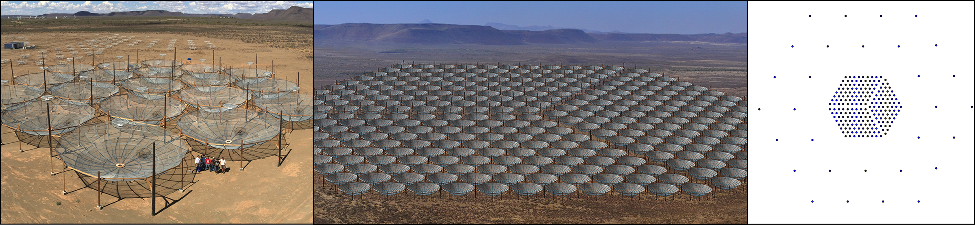
\includegraphics{research_fig.pdf}
\caption{Left: The current 19-element HERA prototype in South Africa.  Center: Rendering of the 331 element HERA core. Right: Proposed HERA configuration including 208 element core (supported under current NSF grant) core and 30 outrigger antennas.}
\label{fig:research}
\vspace{-0.2in}
\end{figure}

\vspace{8pt}
\textbf{Approaches.} Recent work by \cite{dillon_and_parsons_2016} demonstrated how adding a small number of ``outrigger'' antennas at large distances from the HERA core can dramatically improve imaging fidelity and allow reliable calibration to achieve high quality images.  In support of the ENRICH program, the HERA project will add 30 outrigger antennas which will more than triple the resolution of the  array while retaining all of its science capabilities (Fig. \ref{fig:research}; right panel). Given this support from the project (see accompanying letter from HERA project manager Dave DeBoer), ENRICH will undertake the development of the imaging analysis itself, which requires substantial advances in algorithms and software implementation.  Undergraduates, graduate students, and early-career researchers supported under this proposal will contribute primarily to the commissioning of the new instrument capabilities and the design of new data analysis tools to process imaging data at the precision required by 21\, cm cosmology experiments.

\vspace{8pt}
\textbf{Expected Outcomes and Timeline.} The principal research outcome of ENRICH will be the most compelling measurements of the cosmological 21\, cm signal to date.  These measurements can reveal the properties of the first stars and galaxies with per cent level accuracy \citep{pober_et_al_2014,greig_and_mesinger_2015,ewall-wice_et_al_2016}, and, for the first time, we will be able to cross-correlate these measurements with other probes of the early universe to produce a complete picture of our ``cosmic dawn."  All code developed under this project will be open source (shared on GitHub), and all data products will be served to the public through our colleagues at the National Radio Astronomy Observatory (NRAO).  This proposal also enables ancillary science by other groups by producing high quality images for a variety of investigations.

The ENRICH timeline meshes well with the ongoing construction of HERA, which will have 37 antennas operating at the end of 2016, and the fully-funded 208 element core operational by the end of 2018.  There will therefore be useful data appearing in the first year of this grant, and all necessary hardware complete by the end of year two.  The final three years will be dedicated to the development of software and analysis of HERA imaging data.  The tools developed through the ENRICH program are forward-looking and are applicable to third-generation experiments beyond the end of the current HERA project.

\vspace{8pt}
\textbf{The Collaboration.} Brown University, the University of Washington, and the University of Pennsylvania are all executive members of the HERA collaboration and bring expertise in the analysis of 21\, cm cosmology data, as well as their own unique skill sets.  PI Pober pioneered the non-imaging ``delay spectrum" approach with the Precision Array for Probing the Epoch of Reionization (PAPER) and now leads the end-to-end pipeline simulation efforts for HERA.  Co-PI Morales' group at Washington has developed one of the most robust imagers specifically for 21\, cm cosmology in the Fast Holographic Deconvolution software package\footnote{https://github.com/EoRImaging/FHD} and has led the US image-based analysis for the Murchison Widefield Array EoR project.  Co-PI Aguirre at Penn has led the effort to understand polarization systematics in the PAPER and HERA experiments, and brings advanced techniques for mitigating them in both imaging and non-imaging approaches; Penn Co-PI Lidz has been a key player in laying the theoretical groundwork for imaging the 21\,cm signal.  Co-PI Glendenning at the NRAO brings data server and data archive expertise and will facilitate the development of cloud computing (Amazon/XSEDE) as well as the hosting and sharing of public data products.  Lastly, Co-PI Rudolph at Cal Poly is the founder and director of the CAMPARE and CHAMP programs (described in the education statement), and will provide training to our project administrator and help further develop our network with URM-serving community colleges and state universities.

South African collaborators Bernardi, Santos, Sievers, and Smirnov bring a wide variety of forward looking techniques for radio astronomy, image-based 21\, cm analysis, and cosmology from their work with the Murchison Widefield Array (MWA), SKA, and cosmic microwave background experiments.  This proposal will enrich scientific collaboration with the burgeoning South African scientific community, which is nascent but developing rapidly.  South Africa is host to half of the proposed SKA, which will be the world's largest radio telescope. At present, the US has no formal involvement in the SKA, but this proposal would enable ENRICH member institutions to take an international leadership role in the crucial analysis methods and software for the leading science driver of the SKA.

\vspace{8pt}
\textbf{Summary.} ENRICH will provide a significant leap forward in the sophistication of 21\, cm cosmology analysis.  These tools will move the community from a statistical measurement of the overall signal to producing maps of cosmic hydrogen that can be compared with other probes of the early universe.  The result will be a transformation in our understanding of the first stars and galaxies and the processes that molded them into the universe we see today.

\clearpage
\setcounter{page}{1}

\setlength{\parindent}{0cm}
\textbf{\large The Educational Network for Research in Imaging Cosmological Hydrogen}\\
\textbf{Education Statement}
\vspace{6pt}
\setlength{\parindent}{17pt}

The educational component of the ENRICH program consists of three main goals:

\begin{enumerate}
\item To create and promote opportunities for students and early career researchers to participate in substantive international research experiences 
%by funding travel and 
%building on the active integration of 
with South African faculty, students, and postdocs working on HERA (thus addressing the fourth PIRE program objective)
%begun with The Hydrogen Epoch of Reionization Array (HERA).

\item To create an annual international scientific workshop and symposium led by early career researchers (with an emphasis on undergraduate participation) focusing on the scientific exploitation of data from 21\, cm cosmology experiments.

\item To identify underrepresented minorities (URM) at the college level and, based on a successful model of research engagement, increase the number of URM students completing STEM undergraduate degrees and continuing to graduate school.
\end{enumerate}

All three initiatives will be heavily integrated with each other and with the programs being implemented under the HERA grant, as described below, and 
% JA: I don't love this statement any more, as it looks like the PI is abdicating responsibility and is vague.  I also think that research management should be discussed in the research statement.  
%For ENRICH, the project administrator will be primarily responsible for the education component, as the construction is managed through HERA and the scientific collaboration of HERA provides a matrix for administration of the research.
%JCP the following sentence should find a home below
%All three initiatives 
will be directed by a full-time project administrator, ideally with training in physics and/or physics education, whose primary responsibility will be the education component.  


%\vspace{8pt}
\textbf{Approach.} We will work closely with two highly successful programs for increasing the number of URM students in STEM fields: the Leadership Alliance (LA) and the California Arizona Minority Partnership for Astronomy Research and Education (CAMPARE).
The LA is a Brown-based consortium of more than 30 academic and industrial partners
% JA: I was bothered by colleges and universities plural, but industry singular
% leading colleges, universities and private industry 
dedicated to increasing the participation of URM in graduate programs.
%JA: I think redundant, given the next statement , with a long and productive history.  
%The LA aims to create leaders and role models for coming generations by providing undergraduate internships and mentoring; graduate support and fellowships; faculty development opportunities, and research exchanges.  
In its first 20 years, just at Brown alone, the LA mentored more 400 participants, 38 percent of whom received a graduate level degree. CAMPARE, directed by Co-PI Rudolph, has operated for seven years to engage URM and women in authentic research activities, with a very high success rate for graduation and placement in STEM higher education programs.  Currently, CAMPARE has a network of 22 California State Universities and Community Colleges (nearly all official Hispanic-Serving Institutions) from which they draw undergraduate students for placement in summer research programs at some of the leading universities in California and Arizona.  The newly formed CAMPARE-HERA Astronomy Minority Partnership (CHAMP) --- in which Brown, UW, and UPenn are members --- 
%has already begun work to build on CAMPARE and 
taps into this existing network of schools to bring women and URM students into summer research programs with HERA scientists.
\emph{ENRICH will integrate the astronomy-focused techniques of CAMPARE and CHAMP with the nationwide infrastructure for student recruitment and mentoring of the LA to produce a fundamentally new program in collaboration with our South African colleagues.} 

\begin{figure}[!ht]
\centering
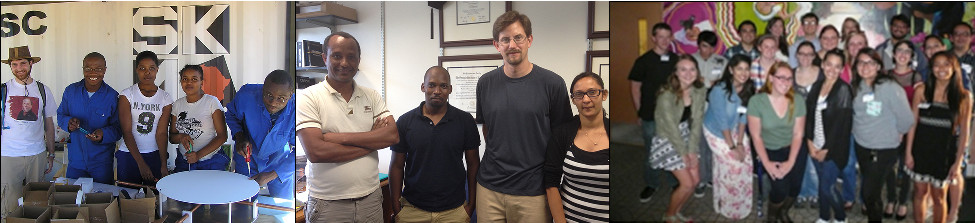
\includegraphics{education_fig.pdf}
\caption{Left: PI Pober and South African students assembling antennas on the HERA site.  Center: Co-PI Aguirre and the first group of South African exchange students (supported under the initial HERA grant) at UPenn.  Right: Students at the 2014 CAMPARE mentoring dinner organized by Co-PI Rudolph.}
\label{fig:education}
\vspace{-0.2in}
\end{figure}

\textbf{Program Outline.} The ENRICH educational program will begin by recruiting five rising-junior undergraduate researchers from around the country for a nine-week summer research experience.  To identify this initial group of students, our full-time project administrator will work closely with the LA and CAMPARE, using their existing network of URM-serving institutions.  Before arriving, these students will be assigned a graduate student mentor who will assist the students in crafting the scope of their research project and serve as a study group leader over the summer.  The first week of the research experience will be an instructional workshop in 21\,cm cosmology and the software tools the students will be using.  In subsequent years, two previous ENRICH students (now rising seniors) will be selected for a second summer research experience in South Africa working under the direct guidance of our collaborators and a graduate student mentor.  Building on their previous experience,
%Since these students have already had a significant research experience in the field, 
they will be well prepared for an impactful, cutting edge research.
% and exciting research project at the cutting edge of ENRICH science.

To remove financial impediments to participation, ENRICH will provide a competitive stipend, housing, and travel.  
%Graduate student mentors will also receive travel support and housing in South Africa.  
ENRICH research students receive year-round mentoring, 
%which has been shown to positively impact 
improving performance, academic self-esteem, and persistence within a major \citep{cross_and_vick_2001,armstrong_and_thompson_2003}. They will also be supported in presenting their research to their peers and at conferences; such opportunities are invaluable for increasing interest in a research career and the likelihood of obtaining a PhD \citep{nsf_report_2006}.
%the 2006 report Evaluation of NSF Support for Undergraduate Research Opportunities.
% JA: I think there can only be one capstone :)
%The capstone events for ENRICH students will be two research symposia: 
%ENRICH students will be actively integrated with collaboration research: 
Mid-summer,  ENRICH students will present 
%their work 
at the LA symposium, which hosts students from all disciplines, and  at the end of the summer, all CHAMP and ENRICH participants (including visiting South African students) will present 
%their work 
at a 21\,cm cosmology symposium with ENRICH mentors, HERA PIs, and other scientists in attendance.  Student presentations are the focus of both symposia.

Initially, the students will be hosted at Brown, drawing on existing LA infrastructure.  
%Over this time, 
The project administrator will work to build a local recruitment network for ENRICH institutions by cultivating contacts at URM serving institutions in New England, Philadelphia and Seattle.  Co-PI Rudolph will assist in these efforts.  
%Ultimately, 
The expanded network will allow UPenn and UW to host summer students in later years of the program.  The connections to local institutions will prove invaluable after the end of the ENRICH program, allowing 
%even if there is no longer funding for cohorts of 5+ students, 
%ENRICH 
PI's to use an established network to continue these efforts in their communities.
% on a smaller scale.
Overall, ENRICH will provide research experiences to 5 - 7 undergraduate students per year. Given the 
%with an 
annual average of only 5 URM PhDs 
%awarded to URM students 
in astronomy, our program can have a national impact on the number of 
%women and 
URM students in astronomy.
%entering graduate programs.

\textbf{Assessment and Evaluation.} 
Brown's Science Center Outreach 
%evaluation resources 
and/or external evaluators
%Assessment of the educational component 
will 
%not only 
assess the impact of the educational initiatives for reporting purposes and also to improve the quality of these efforts. %over the 5-year span of the PIRE award.  
We will assess 
%multiple domains of 
students' learning outcomes, including cognition, 
%(what do learners know?), 
process,
% (what can learners do?), 
and affect 
%(what are learners attitudes?) 
using pre- and post- measurement tools.
% whenever possible.  
ENRICH mentors will also 
%continue to 
remain in contact
% beyond graduation 
to understand how ENRICH experiences affected scholars' education and career decisions.
Evaluation will also assess the recruitment, retention, and success of ENRICH scholars by tracking 
%metrics such scholar 
diversity and numbers %of scholars 
completing college and graduate school.  

\textbf{Summary.} The integration of research and education in ENRICH will produce a unique program that accomplishes more than either aspect on its own.  The international nature of the education program provides students with truly engaging experiences with a cutting edge experiment.  The research program strongly benefits from the inclusion of young and underrepresented students as well, as ENRICH will ultimately train a diverse group of researchers to lead the next generation of experiments.  

\clearpage
\setcounter{page}{1}
\thispagestyle{empty}
\bibliographystyle{jponew}
\bibliography{masterbib}

\end{document}

